\chapter{Imlement algorithm for training weigths for vector association measure}

\section{Algorithms implemented in MeWeX}
MeWeX contains several algorithms which were implemented by Łukasz Kłyk in his \(Optimizer\) and adopted by 
Michał Wendelberger.

TODO

% Wagi rankingów to parametry algorytmu kombinacji, które powinny zostać wyznaczone eks-
% perymentalnie, na przykład poprzez ich optymalizację. Prezentowane oprogramowanie umożli-
% wia wykorzystanie do tego celu pięciu różnych algorytmów heurystycznych i metaheurystycz-
% nych implementacji Łukasza Kłyka [13]. Utworzony przez niego Optimizer został przystoso-
% wany przez autora niniejszej pracy do działania z opisywanym MWeXtractorem. Łukasz Kłyk
% zaimplementował następujące algorytmy w swoim oprogramowaniu:

% Nazwy wspomnianych algorytmów heurystycznych i metaheurystycznych dokładnie określa-
% ją, jakie są to algorytmy, jednak poza dwoma wyjątkami – symulowanym wyżarzaniem i algoryt-
% mem ewolucyjnym. Pierwszy z nich nie precyzuje schematu chłodzenia, ale domyślnie w opro-
% gramowaniu zaimplementowanym przez Łukasza Kłyka stosowana jest funkcja T (k) = 0.3 k
% [13, str. 36]. Przypadek algorytmu ewolucyjnego wymaga dłuższego opisu, ponieważ pojęcie to
% jest znacznie szersze od nazw pozostałych metod.


\begin{itemize}
    \item \textbf{Evolutionary Algorithm} - Description
 
    \item \textbf{Hill Climbing} - Description
 
    \item \textbf{Tabu Search} - Description
 
    \item \textbf{Random Search} - Description
 
    \item \textbf{Simulated Annealing} - Description 
\end{itemize}

\section{Particle Swarm Optimization}

\subsection{Description}
Particle Swarm Optimization is an algorithm for optimization of a problem. It tries to improve a candidate solution 
accordingly to a given measure of quality. PSO have population of particles called swarm and solves problem by iteratively moving those particles 
through the search space using formula that involves particle velocity, local best solution and global best solution. 

Algorithm starts with placing all particles in search space choosing random uniformly distributed positions for them and initializing its velocity to 0. 
Then for first particle solution is evaluated, next it assigns its starting position as a local and global best position. 
This step is repeated for all particles in the swarm, but global best position is changed only when new one achieves higher score. 
From that point all steps are performed in a loop till stop condition will not be satisfied. For every paricle, at first 
velocity is updated, then its position is changed by the velocity vector and quality of new position is evaluated. 
If new score is is higher than local or global best, then they are updated accordingly. When algorithm reaches stop conition 
then position of global best solution is returned as a result.
In the figure \ref{pso_flowchart} there is presented flow chart of Particle Swarm Optimization.
\begin{figure}[ht]
    \centering
    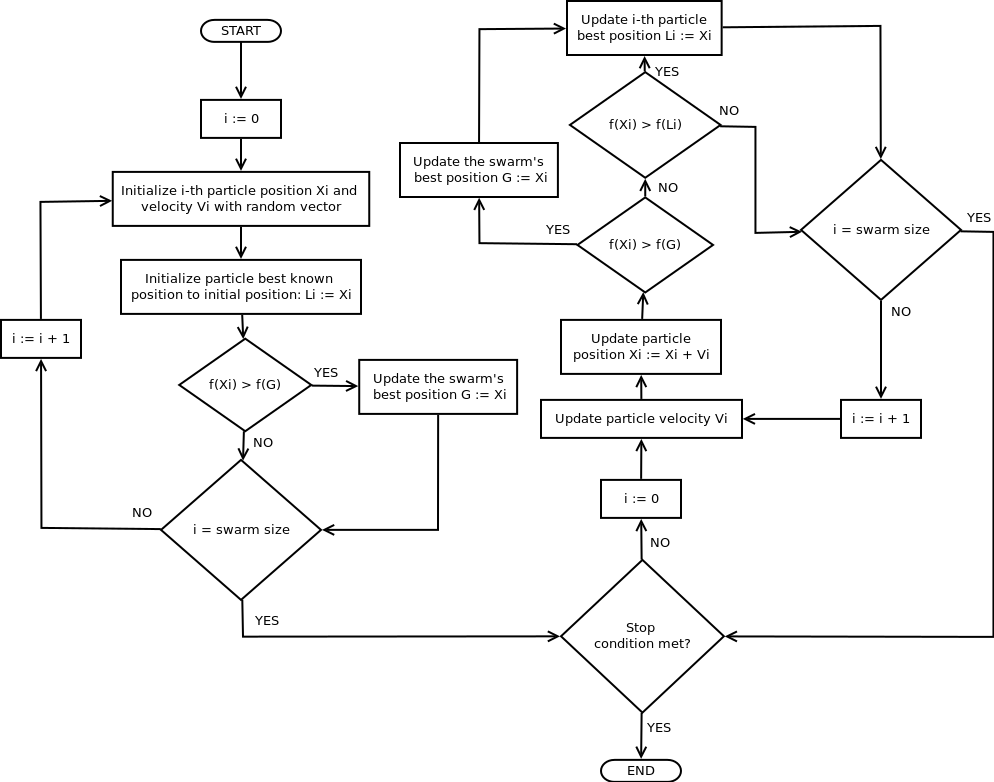
\includegraphics[scale=0.4]{img/pso_flowchart.png}
    \caption{Flow chart of Particle Swarm Optimization}
    \label{pso_flowchart}
\end{figure}

Particles move toward local and global maxima making swarm more dense in surroundings of best known positions. 
That property entail swarm for searching better solutions.
Below there is formula for updating velocity of the particles.
\[ 
    V \gets \omega V + \omega _{p} r _{p} (p - x) + \omega _{g} r _{g} (g - x)
\]
Where: \\
\(V\)  - velocity of given particle, it is vector of size equal to number of dimensions in search space \\
\(r _{p}, r _{g}\) - random numbers from interval \((0,1)\) \\
\(\omega, \omega _{p}, \omega _{g}\) - parameters, chosen by the user, which controls behaviour of the PSO \\
\(x\)  - position of given particle \\
\(p\)  - position of best solution achieved by given particle \\
\(g\)  - position of global best solution achieved by the swarm \\

One of the factor for calculating new velocity is its previous value. Preserving partially old velocity makes particle behavior 
like it would have momentum, smoothing its movement. Particle aims toward global and local best, but force of those both factors is randomized.
New velocity is composed from three vectors and strength of influence for each of them can be adjusted by changing value 
of corresponding \(\omega\) parameter. By modifing those parameters it is possible to control behavior of the swarm, for example 
by reducing momentum or increasing importance of local maxima.

Particle Swarm Optimization is quite simple algorithm, but it can achieve good result. Its simplicity allows easy modification and adjusting 
algorithm for needs of the user. It has three parameters that can influence behavior of the swarm, but their tuning is intuitive. 
Disadvantage of this algorithm is that it has tendency to fall in the local maxima. Next problem is that for high dimensional search spaces 
swarm has to be more populated what greatly increases computational time. 

\subsection{Motivation}
One of the method to increase efficiency of the MeWeX was to improve selection of weigths for aggregators. 
Implementing new algorithm Particle Swarm Optimization was reasonable solution taking into account its simplicity 
connected with good efficacy. Susceptibility on modifications and easy adjustment of parameters make it also a good choice.

\subsection{Implementation}
Expanded structure and modular architecture of MeWeX made simple further extensions of code. Class diagram presented on figure \ref{img_pso_class}
presents the structure of implemented algorithm.
\begin{figure}[ht]
\centering
    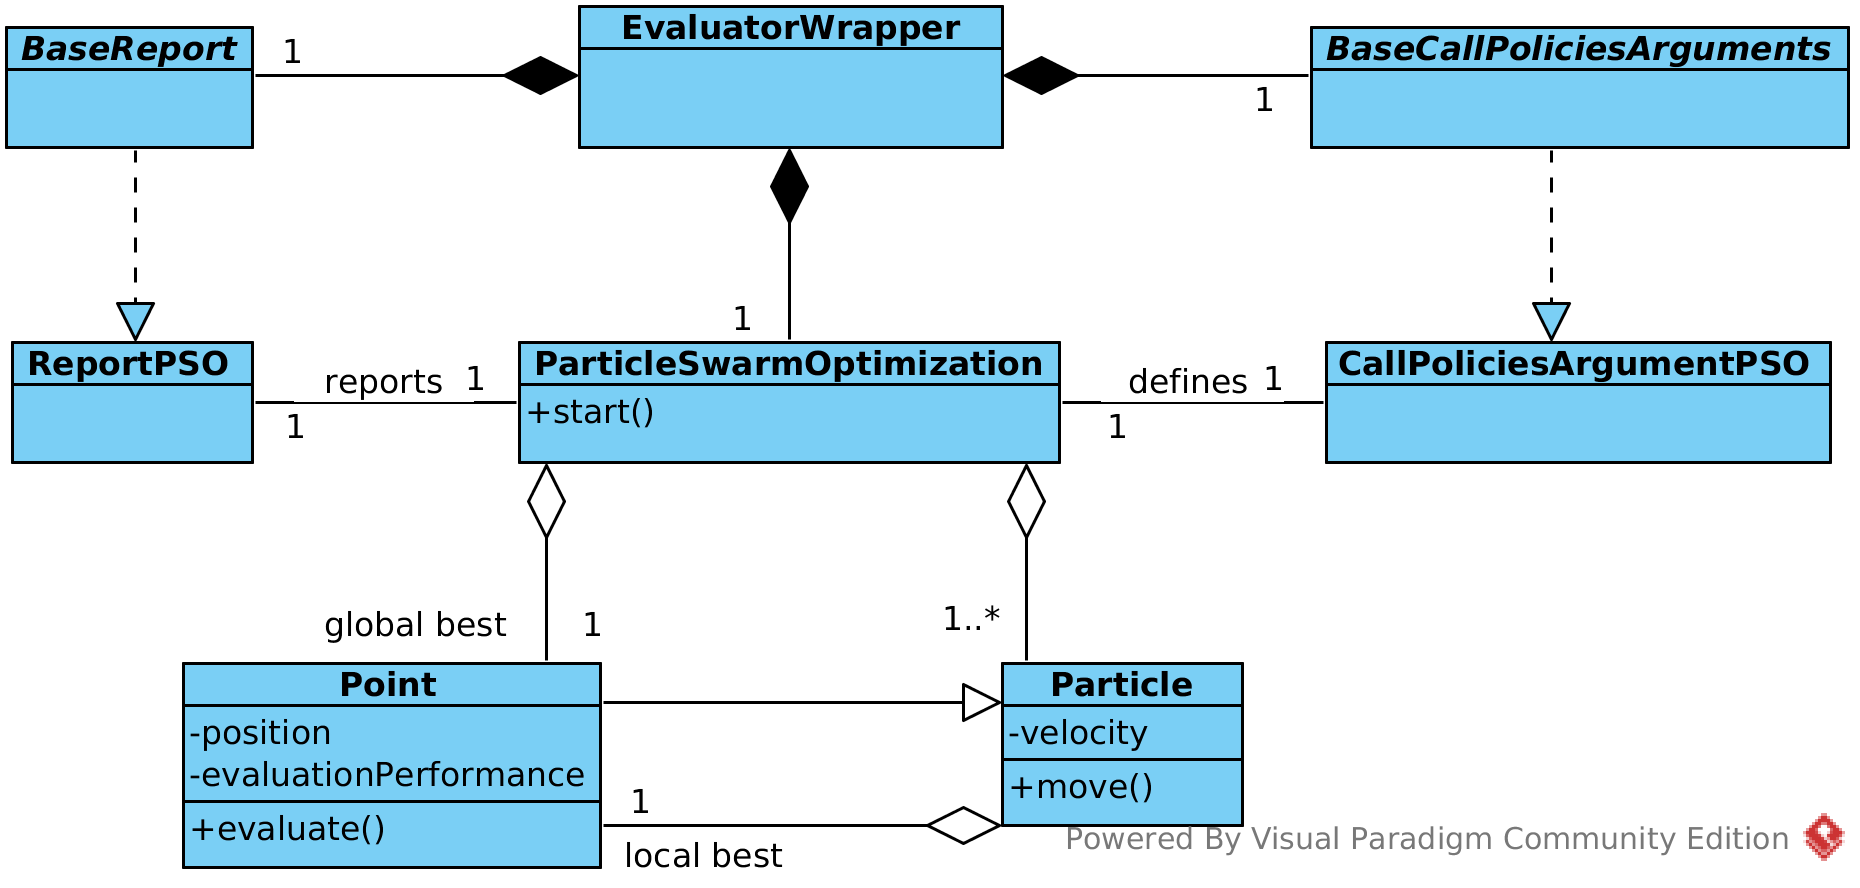
\includegraphics[scale=0.5]{img/pso_class.png}
    \caption{Class diagram of Particle Swarm Optimization}
    \label{img_pso_class}
\end{figure}


To make possible using new algorithm in the same way as already implemented few steps was neccesary to perform.
At first, class \(ParticleSwarmOptimization\) had to be created base on implementation of other machine learning algorithms. 
It does not need to inherit any other class, but it has to be template class, with the same set of template parameters like in other classes. 
Next requirement is that it must define constructor \textit{ParticleSwarmOptimization(const Point\& rStartPoint, Evaluator* pEvaluator, const ArgumentsType\& rArgs)} 
and fuction \(Point\ start()\) which executes whole algorithm and returns best found solution.
Next step was to implement two classes, one which inherits by \(BaseCallPoliciesArguments\) and defines parameters that can be passed by user, 
and second which inherits by \(BaseReport\) and specifies format of creating report of training, which is written to file during algorithm work.
Then, those classes had to be added to \(EvaluatorWrapper\) which is responsible for running chosen algorithm, 
passing arguments from user and creating report. Code below shows modification of that class, where PSO was added.
\begin{lstlisting}
class EvaluatorWrapper
{
public:

        ...

    typedef particle_swarm_optimization::CallPoliciesArgumentsPSO	PSOCallPolicy;

    enum MethodType
    {
        ...

        PSO,  // Particle Swarm Optimization
        EMPTY
    };
        ...

    EvaluatorWrapper(
        EvaluatorPtrR const&	pEvaluator,
        MethodType              pMethodType,
        Point const&	        pStartPoint,
        PSOCallPolicy const& 	pPolicy);

        ...
    
    void setParticleSwarmOptimizationPolicy(PSOCallPolicy const& pPolicy);

private:
        ...
    
    PSOCallPolicy mPSOCPA;
};
\end{lstlisting}
    
% \begin{lstlisting}
%         ...

% EvaluatorWrapper::EvaluatorWrapper(
%     EvaluatorPtrR const&	pEvaluator,
%     MethodType 			pMethodType,
%     Point const&		pStartPoint,
%     PSOCallPolicy const& 	pPolicy)
% :
%     mMethodType(pMethodType),
%     mStartPoint(pStartPoint),
%     mEvaluator(pEvaluator),
%     mPSOCPA(pPolicy)
% {}

% auto EvaluatorWrapper::parseMethodType(std::string const& pMethod) -> MethodType
% {
%     if(boost::iequals(pMethod, "RS"))
%     {
%         return RS;
%     }    
    
%         ...
        
%     else if(boost::iequals(pMethod, "PSO"))
%     {
%         return PSO;
%     }
%         ...

% void EvaluatorWrapper::setParticleSwarmOptimizationPolicy(PSOCallPolicy const& pPolicy)
% {
%     mPSOCPA = pPolicy;
% }

% auto EvaluatorWrapper::start() -> Point
% {
%         ...

% typedef particle_swarm_optimization::ParticleSwarmOptimization<
%             particle_swarm_optimization::CallPoliciesArgumentsPSO,
%             unsigned int,
%             Step,
%             time_t,
%             Timer,
%             particle_swarm_optimization::ReportPSO> PSOAlgorithm;

%         ...

% switch(mMethodType)
% {
%         ...
        
%     case PSO:
%     {
%         return PSOAlgorithm(mStartPoint, mEvaluator, mPSOCPA).start();
%     }
%     break;

%         ...
% \end{lstlisting}
Last step is to implement algorithm itself, but it needs a class that represents particle and MeWeX machine learning module implements only class \(Point\).
Class \(Particle\) was created by author of this thesis by inheriting class \(Point\), adding velocity vector and best local position and defining 
function \(void\ move(const\ Point\&\ rBest)\).
% \begin{lstlisting}
% void Particle::move(const Point& rBest)
% {
%     double c1 = 1.0, c2 = 0.2, c3 = 0.8;
%     double r1 = Random::random(), r2 = Random::random(), r3 = Random::random();
%     for(int i = 0; i < mVelocity.size(); i++)
%     {
%         double v,mX,rX,cX;
%         auto data = mVelocity[i]->getValueAt(0);
%         mVelocity[i]->getValueAt(0).get(v);
%         mBest->getParameterAt(i).getValueAt(0).get(mX);
%         mParameters[i]->getValueAt(0).get(cX);
%         rBest.getParameterAt(i).getValueAt(0).get(rX);
%         v = (c1 * r1 * v) + (c2 * r2 * (mX - cX)) + (c2 * r2 * (rX - cX));
%         data.set(v);
%         mVelocity[i]->setValueAt(0, data);
%         data.set(cX + v);
%         mParameters[i]->setValueAt(0, data);
%     }
% }
% \end{lstlisting}
Having implemented class \(Particle\) it was possible to write fuction \(Point\ start()\) which executes algorithm. 



\subsection{Improvements}\label{pso_improv}
Initial investigation of algorithm work showed that algorithm improves the score at early stage of work, but then it finds local maximum 
and stops seeking for better solutions. It was caused by the situation where all particles reached the position between 
local and global best solution, so their velocity lowered to values close to zero. Figure \ref{img_pso_imp_plot1} shows the quality of solution 
during algorithm work, where it is visible how swarm has fallen in local maximum and make no progress.
\begin{figure}[ht]
\centering
	\includegraphics[scale=0.5]{img/pso_imp_plot1.png}
	\caption{Plot of PSO algorithm }
	\label{img_pso_imp_plot1}
\end{figure}

To prevent that issue author of this thesis proposed a function which reallocates all particles when algorithm encounter that problem. 
To detect when swarm stopped search, it calculates sum of velocity vector length of all particles. 
If that sum drops below some specified value, function, which places all particle in random position is called. 
\begin{figure}[ht]
	\centering
	\includegraphics[scale=0.5]{img/pso_imp_plot2.png}
	\caption{Plot of PSO algorithm }
	\label{img_pso_imp_plot2}
\end{figure}

Second problem with PSO was that search space had a lot of dimensions, and by reason of long computation time to evaluate single particle solution, 
size of the swarm was limited. This caused that only small part of search space was explored. Solution of that problem, 
proposed by the author of this thesis was to change the distribution of starting positions. Instead of uniform distribution, positions was randomized 
with more problability beeing close to edge. This distibution is presented on figure \ref{img_pso_imp_dist}.

\begin{figure}[ht]
	\centering
	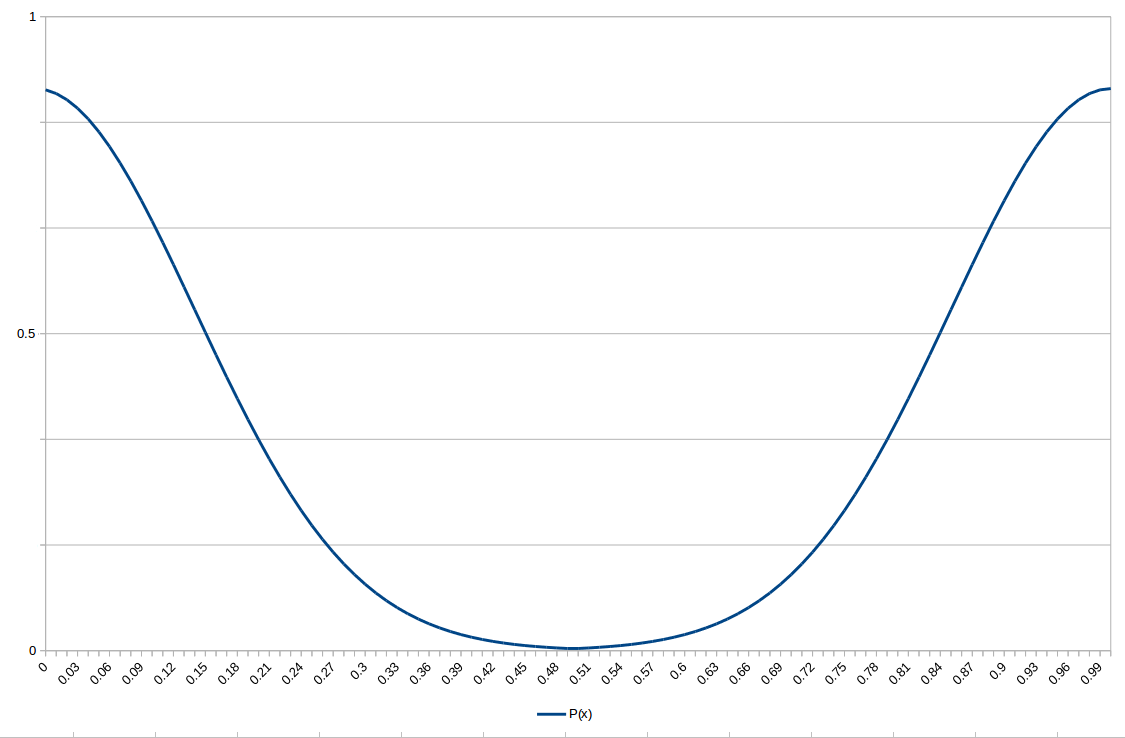
\includegraphics[scale=0.4]{img/pso_dist.png}
	\caption{Probability distribution for selecting particle position}
	\label{img_pso_imp_dist}
\end{figure}

For creation of that probability distribution there was used class, provided by C++11 Standard Library, 
\textit{template< class RealType = double > class normal\_distribution;} which produces random numbers with normal probability
with specified mean and standard deviation. Method, which converts normal distribution to the shown on the plot in the figure \ref{img_pso_imp_dist} 
is shown below.

\begin{lstlisting}
std::normal_distribution<double> Random::normal(0.5, 0.1);
std::mt19937_64 Random::generator(time(nullptr));

double Random::random_inv_normal(void)
{
    double val = normal(generator);
    if(val < 0.5)
    {
        val += 0.5;
        if(val < 0)
            val = 0;
    }
    else
    {
        val -= 0.5;
        if(val > 1)
            val = 1;
    }
    return val;
}
\end{lstlisting}